\section{Expected Event Rate and Oscillation Parameters}
%{\it Assigned to:} {\bf Mayly Sanchez} 
\label{sec:physics-lbnosc-osc}


The oscillation probability of \numu $\rightarrow$ \nue through matter in a constant density
approximation is,  % Anne 3/9
to first order~\cite{Nunokawa:2007qh}:
%
\begin{eqnarray}
P(\nu_\mu \rightarrow \nu_e) & \simeq & \sin^2 \theta_{23} \sin^2 2 \theta_{13} 
\frac{ \sin^2(\Delta_{31} - aL)}{(\Delta_{31}-aL)^2} \Delta_{31}^2\\ \nonumber
& & + \sin 2 \theta_{23} \sin 2 \theta_{13} \sin 2 \theta_{12} \frac{ \sin(\Delta_{31} - aL)}{(\Delta_{31}-aL)} \Delta_{31} \frac{\sin(aL)}{(aL)} \Delta_{21} \cos (\Delta_{31} + \mdeltacp)\\ \nonumber
& & + \cos^2 \theta_{23} \sin^2 2 \theta_{12} \frac {\sin^2(aL)}{(aL)^2} \Delta_{21}^2, \\ \nonumber
\label{eqn:appprob}
\end{eqnarray}
where $\Delta_{ij} = \Delta m^2_{ij} L/4E_\nu$, $a = G_FN_e/\sqrt{2}$, $G_F$ is the Fermi constant, $N_e$ is the number density of electrons in the Earth, $L$ is the baseline in km, and $E_\nu$ is the neutrino energy in GeV. 
In the equation above, both \deltacp and $a$ 
switch signs in going from the
$\nu_\mu \to \nu_e$ to the $\bar{\nu}_\mu \to \bar{\nu}_e$ channel; i.e.,
a neutrino-antineutrino asymmetry is introduced both by CP violation (\deltacp)
and the matter effect ($a$). The origin of the matter effect asymmetry 
is simply the presence of electrons and absence of positrons in the Earth.  
In the few-GeV energy range, the asymmetry from the matter effect increases with baseline as the neutrinos
pass through more matter, therefore an experiment with a longer baseline will be
more sensitive to the neutrino mass hierarchy. For baselines longer than 
$\sim$\SI{1200}\km, the degeneracy between the asymmetries from matter
and CP-violation effects can be resolved~\cite{Bass:2013vcg}; hence DUNE, with a baseline of $\sim$\SI{1300}\km, 
will be able to unambiguously
determine the neutrino mass hierarchy \textit{and} measure the value of \deltacp~\cite{Diwan:2004bt}. 

The electron neutrino appearance probability, $P(\nu_\mu \rightarrow \nu_e)$, 
is shown in 
Figure~\ref{fig:oscprob} \todo{Figure 3.1 from CDR here}
at a baseline of \SI{1300}\km{} as a function of neutrino 
energy for several values of \deltacp. As this figure illustrates, the value 
of \deltacp affects both the amplitude and frequency of
the oscillation. The difference in probability amplitude
for different values of \deltacp is larger at higher oscillation nodes, which 
correspond to energies less than 1.5~GeV. Therefore, a broadband experiment, 
capable of measuring not only the rate of \nue appearance but of mapping out the 
spectrum of observed oscillations down to energies of at least 500~MeV, 
is desirable~\cite{Diwan:2003bp}. Since there are terms proportional to $\sin\mdeltacp$ in Equation~\ref{eqn:appprob},
changes to the value of \deltacp induce opposite changes to \nue and
\anue appearance probabilities, so a beam that is capable of operating in
neutrino mode (forward horn current) and antineutrino mode (reverse horn current)
is also a critical component of the experiment.



\begin{figure}
  \centering
%    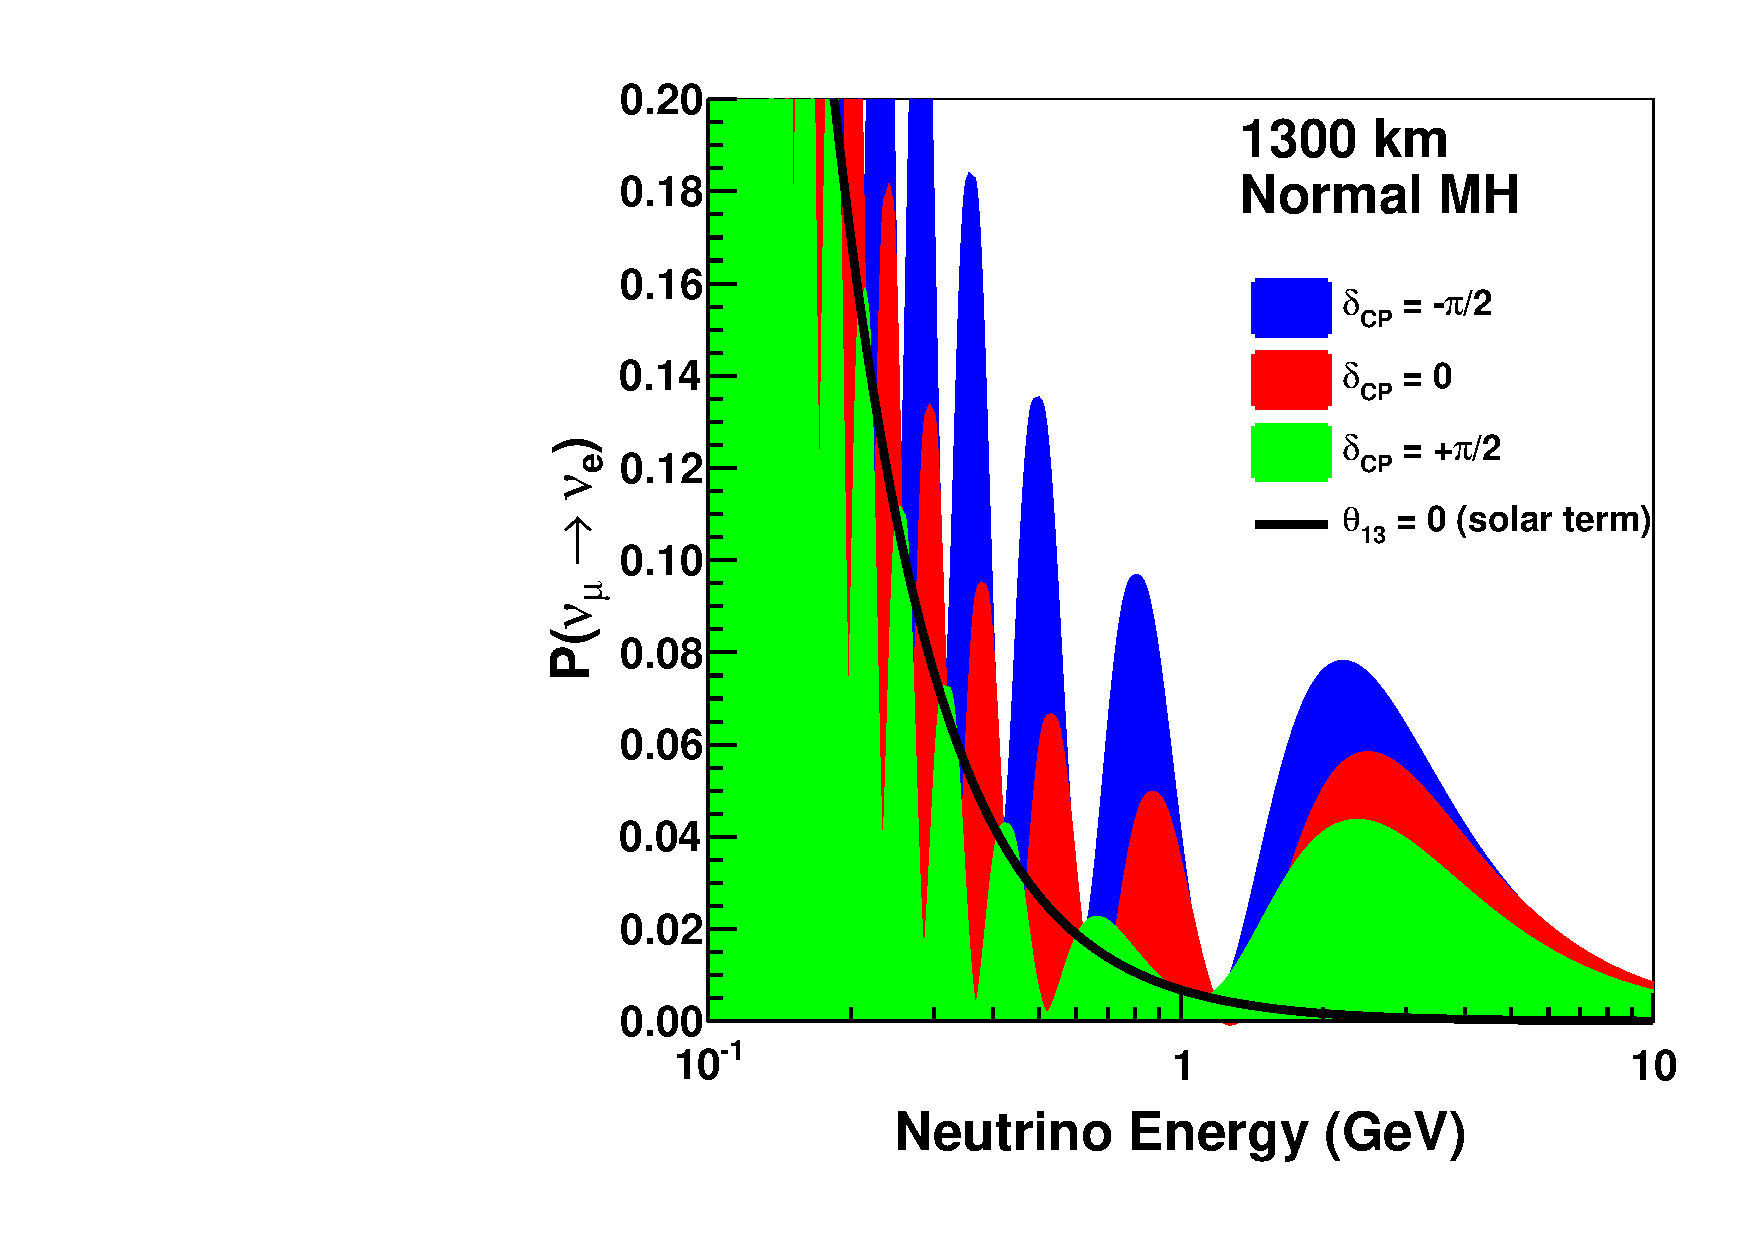
\includegraphics[width=0.45\linewidth]{energy_nu_no.pdf}
%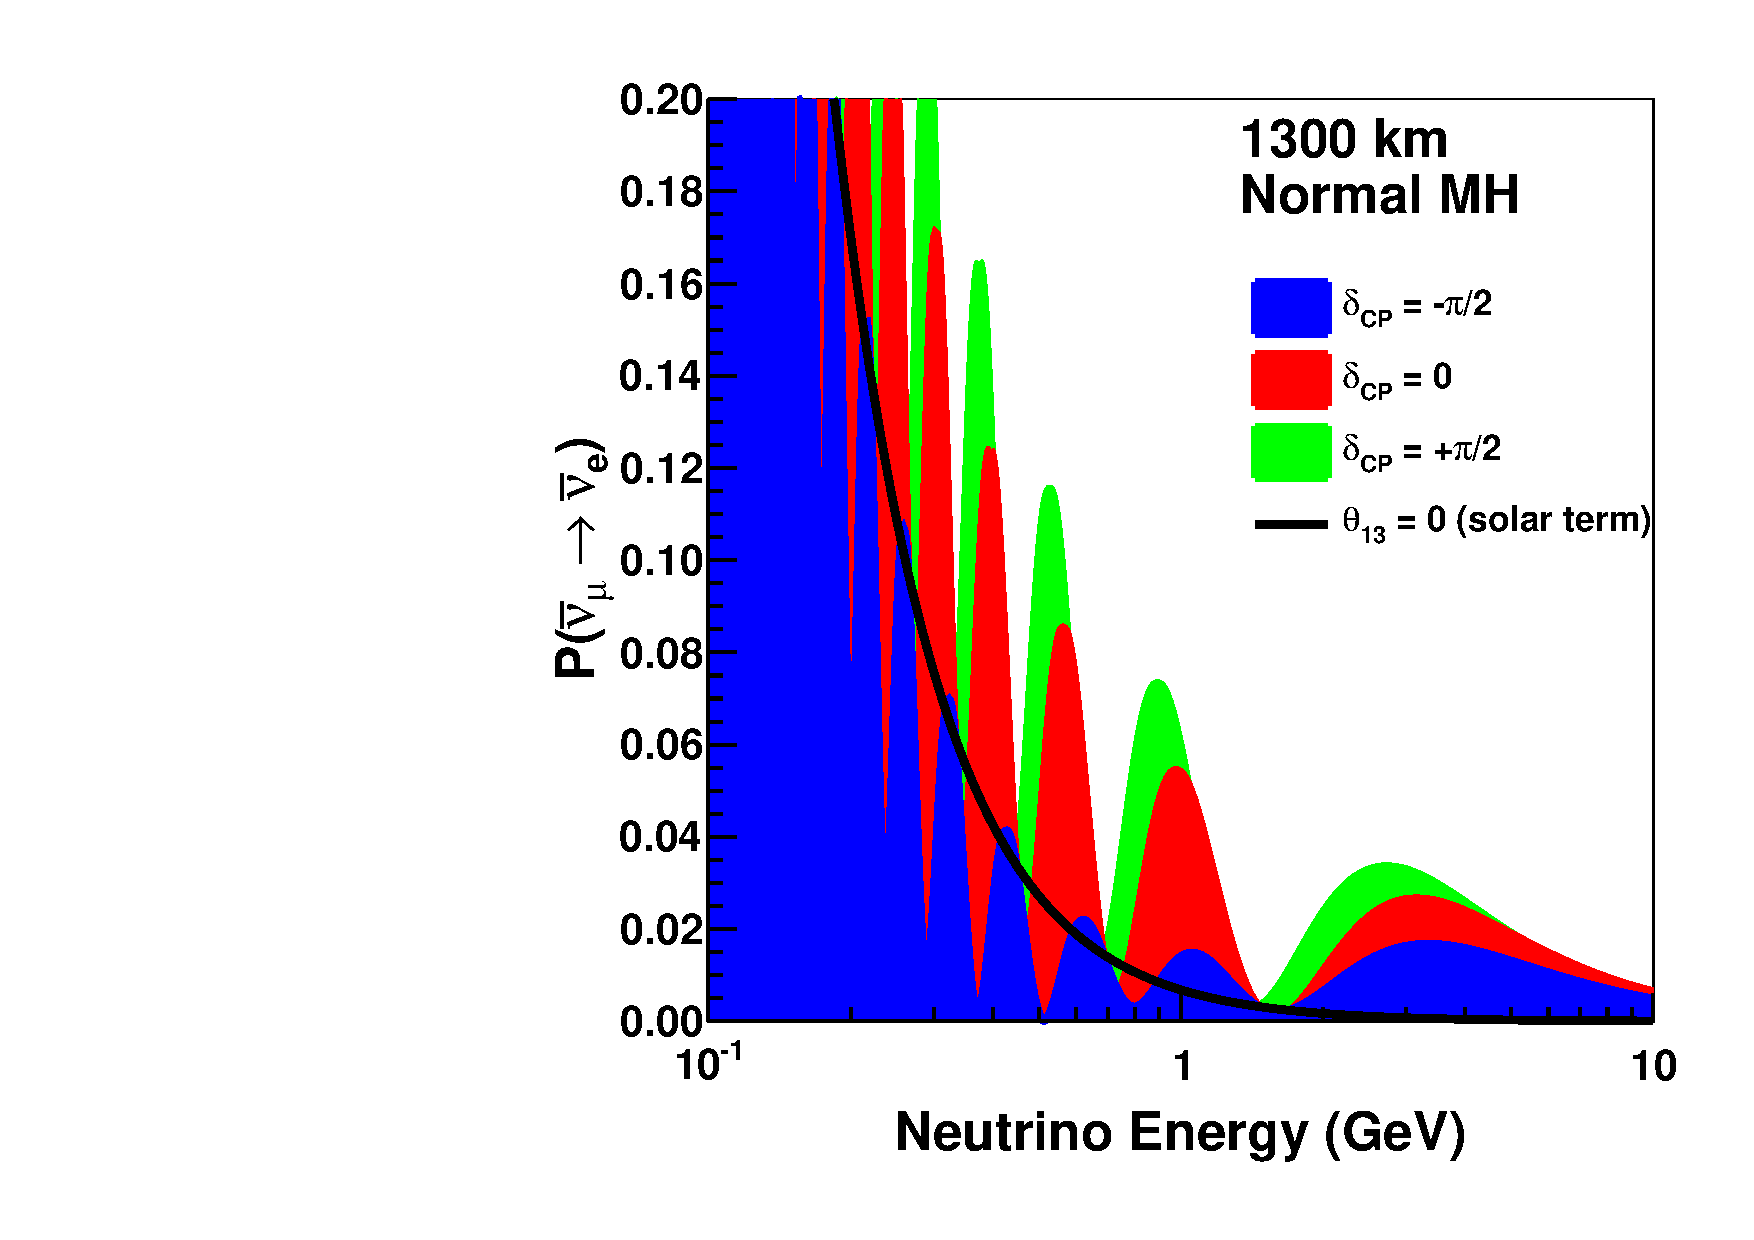
\includegraphics[width=0.45\linewidth]{energy_anu_no.pdf}
  \caption{The appearance probability at a baseline of 1300~km,
  as a function of neutrino energy, for \deltacp = $-\pi/2$ (blue), 
  0 (red), and $\pi/2$ (green), for neutrinos (left) and antineutrinos
  (right), for normal hierarchy. The black line indicates the oscillation
  probability if $\theta_{13}$ were equal to zero.}
  \label{fig:oscprob}
\end{figure}

The experimental sensitivities presented here are estimated using the methods described in Section~\ref{sec:physics-lbnosc-sens}. This document presents physics sensitivities using the optimized design of the 1.2~MW neutrino beam and corresponding protons-on-target per year assumed to be 1.1 $\times 10^{21}$ POT.  These numbers assume a combined uptime and efficiency of the FNAL accelerator complex and the LBNF beamline of 56\% \todo{Check POT per year and uptime efficiency...ETW confirmed}.  The beam design, simulation and associated uncertainties are described in Section~\ref{sec:physics-lbnosc-flux}.

The signal for \nue appearance is an excess of charged-current (CC) \nue and \anue interactions over the expected background in the far detector.  The background to \nue appearance is composed of: (1) CC interactions of \nue and \anue intrinsic to the beam; (2) misidentified \numu and \anumu CC events; (3) neutral current (NC) backgrounds and (4) $\nu_\tau$ and $\bar{\nu}_\tau$ CC events in which the $\tau$'s decay leptonically into electrons/positrons. NC and $\nu_\tau$ backgrounds are due to interactions of higher-energy
neutrinos but they contribute to backgrounds mainly at low energy, which is important for the sensitivity to CP violation.

The Near and Far assumed detector performance parameters are described in detail in Sections~\ref{sec:physics-lbnosc-ND} and~\ref{sec:physics-lbnosc-FD}. A full simulation chain that includes the beam flux, the GENIE neutrino interaction
generator~\cite{Andreopoulos:2009rq}, and Geant4-based detector models has been implemented. 
The reconstruction and particle identification in the Far Detector has also been fully implemented as described in Section~\ref{sec:physics-lbnosc-FD}. For the Near Detector a parameterized reconstruction based on true energy deposits in the active detector volumes has been used as described in Section~\ref{sec:physics-lbnosc-ND}. The neutrino interaction model has been generated using GENIE 2.12 and the choices of models and tunes as well as associated uncertainties are described in detail in Section~\ref{sec:physics-lbnosc-nuint}.

The neutrino oscillation parameters and the uncertainty on those parameters are taken from the Nu-Fit~\cite{Gonzalez-Garcia:2014bfa} \todo{This reference and table needs to be updated} global fit to neutrino data; the
values are given in Table~\ref{tab:oscpar_nufit}.  (See also
\cite{Capozzi:2013csa} and \cite{Forero:2014bxa} for other recent global fits.) Most of the sensitivities in this chapter are shown assuming normal hierarchy; this is an arbitrary choice for simplicity of presentation.

%\begin{cdrtable}[Oscillation parameter values and relative uncertainties]{lcc}{oscpar_nufit}{Central value and relative uncertainty of neutrino oscillation parameters from a global fit~\cite{Gonzalez-Garcia:2014bfa} to neutrino oscillation data. Because the probability distributions are somewhat non-Gaussian (particularly for $\theta_{23}$), the relative uncertainty is computed using 1/6 of the 3$\sigma$ allowed range from the fit, rather than the 1$\sigma$ range.   For $\theta_{23}$ and $\Delta m^2_{31}$, the best-fit values and uncertainties depend on whether normal mass hierarchy (NH) or inverted mass hierarchy (IH) is assumed.}
\begin{table}[]
    \centering
    \begin{tabular}{lcc}
 Parameter &    Central Value & Relative Uncertainty \\
\toprowrule
$\theta_{12}$ & 0.5843 & 2.3\% \\ \colhline
$\theta_{23}$ (NH) & 0.738  & 5.9\% \\ \colhline
$\theta_{23}$ (IH) & 0.864  & 4.9\% \\ \colhline
$\theta_{13}$ & 0.148  & 2.5\% \\ \colhline
$\Delta m^2_{21}$ & 7.5$\times10^{-5}$~eV$^2$ & 2.4\% \\ \colhline
$\Delta m^2_{31}$ (NH) & 2.457$\times10^{-3}$~eV$^2$ &  2.0\% \\ \colhline
$\Delta m^2_{31}$ (IH) & -2.449$\times10^{-3}$~eV$^2$ &  1.9\% \\
    \end{tabular}
    \caption{Central value and relative uncertainty of neutrino oscillation parameters from a global fit~\cite{Gonzalez-Garcia:2014bfa} to neutrino oscillation data. Because the probability distributions are somewhat non-Gaussian (particularly for $\theta_{23}$), the relative uncertainty is computed using 1/6 of the 3$\sigma$ allowed range from the fit, rather than the 1$\sigma$ range.   For $\theta_{23}$ and $\Delta m^2_{31}$, the best-fit values and uncertainties depend on whether normal mass hierarchy (NH) or inverted mass hierarchy (IH) is assumed.}
    \label{tab:oscpar_nufit}
\end{table}
%\end{cdrtable}

Figures~\ref{fig:appspectra} and~\ref{fig:disspectra} show the expected event rate for \nue appearance and \numu disappearance, respectively, including expected flux, cross section, and oscillation probabilities as a function of neutrino energy at a baseline of
\num{1300}~km. The spectra are shown for a \SI{150}~\ktMWyr{} exposure each for neutrino and antineutrino beam mode, for a total \SI{300}~\ktMWyr{} exposure.  The optimized beam design results in an increased signal rate in the lower-energy region. Tables~\ref{tab:apprates} and~\ref{tab:disrates} give the integrated rate for the $\nu_e$ appearance and $\nu_\mu$ disappearance spectra, respectively \todo{Calculate new rates}.  

\begin{dunefigure}[\nue and \anue appearance spectra]{fig:appspectra}
{\nue and \anue appearance spectra: Reconstructed energy distribution of selected $\nu_e$ CC-like events assuming a \SI{150}~\ktMWyr{} exposure in the neutrino-beam mode (left) and antineutrino-beam mode (right), for a total \SI{300}~\ktMWyr{} exposure.  The plots assume normal mass hierarchy and $\mdeltacp = 0$.}
 % \includegraphics[width=0.49\textwidth]{NueApp_NH.pdf}
 %\includegraphics[width=0.49\textwidth]{NueBarApp_NH.pdf}
\end{dunefigure}



\begin{dunefigure}[\numu and \anumu disappearance spectra]{fig:disspectra}
{\numu and \anumu disappearance spectra: Reconstructed energy distribution of selected $\nu_{\mu}$ CC-like events assuming a \SI{150}~\ktMWyr{} exposure in the neutrino-beam mode (left) and antineutrino-beam mode (right), for a total \SI{300}~\ktMWyr{} exposure.  The plots assume normal mass hierarchy and $\mdeltacp = 0$. }
% \includegraphics[width=0.49\textwidth]{NumuDis.pdf}
% \includegraphics[width=0.49\textwidth]{NumuBarDis.pdf}
\end{dunefigure}

%\begin{cdrtable}[\nue and \anue appearance rates]{lcc}{apprates}{\nue and \anue appearance rates: Integrated rate of selected $\nu_e$ CC-like events between 0.5 and 8.0~GeV assuming a \SI{150}~\ktMWyr{} exposure in the neutrino-beam mode and antineutrino-beam mode.  The signal rates are shown for both normal mass hierarchy (NH) and inverted mass hierarchy (IH), and all the background rates assume normal mass hierarchy.  All the rates assume $\mdeltacp = 0$, and the rates are shown for both the CDR reference beam design and the optimized beam as described in Section~\ref{sec:physics-lbnosc-beam-req}.}


\begin{dunetable}
[\nue and \anue appearance rates]
{lrr}
{tab:apprates}
{\nue and \anue appearance rates: Integrated rate of selected $\nu_e$ CC-like events between 0.5 and 8.0~GeV assuming a \SI{150}~\ktMWyr{} exposure in the neutrino-beam mode and antineutrino-beam mode.  The signal rates are shown for both normal mass hierarchy (NH) and inverted mass hierarchy (IH), and all the background rates assume normal mass hierarchy.  All the rates assume $\mdeltacp = 0$.}
& CDR Reference Design & Optimized Design\\ \toprowrule
 $\nu$ mode (\SI{150}~\ktMWyr{}) & & \\
 \colhline 
 \nue Signal NH (IH) & 861 (495) & 945 (521)\\
 \anue Signal NH (IH) & 13 (26) & 10 (22)\\
  \colhline
 Total Signal NH (IH) & 874 (521) & 955 (543) \\
  \colhline 
 Beam $\nu_{e}+\bar{\nu}_{e}$ CC Bkgd & 159 & 204 \\
 NC Bkgd & 22 & 17 \\
 $\nu_{\tau}+\bar{\nu}_{\tau}$ CC Bkgd & 42 & 19 \\
 $\nu_{\mu}+\bar{\nu}_{\mu}$ CC Bkgd & 3 & 3 \\
  \colhline
 Total Bkgd & 226 & 243 \\
 \toprowrule
 $\bar{\nu}$ mode (\SI{150}~\ktMWyr{}) & & \\
 \colhline 
 \nue Signal NH (IH) & 61 (37) & 47 (28)\\
 \anue Signal NH (IH) & 167 (378) & 168 (436)\\
  \colhline
 Total Signal NH (IH) & 228 (415) & 215 (464) \\
  \colhline 
 Beam $\nu_{e}+\bar{\nu}_{e}$ CC Bkgd & 89 & 105 \\
 NC Bkgd & 12 & 9 \\
 $\nu_{\tau}+\bar{\nu}_{\tau}$ CC Bkgd & 23 & 11 \\
 $\nu_{\mu}+\bar{\nu}_{\mu}$ CC Bkgd & 2 & 2 \\
  \colhline 
 Total Bkgd & 126 & 127 \\
\end{dunetable}


%\end{cdrtable}

%\begin{cdrtable}[\numu and \anumu disappearance rates]{lcc}{disrates}{\numu and \anumu disappearance rates: Integrated rate of selected $\nu_{\mu}$ CC-like events between 0.5 and 20.0~GeV assuming a \SI{150}~\ktMWyr{} exposure in the neutrino-beam mode and antineutrino-beam mode.  The rates are shown for normal mass hierarchy and $\mdeltacp = 0$, and the rates are shown for both the CDR reference beam design and the optimized beam as described in Section~\ref{sec:physics-lbnosc-beam-req}.}

\begin{dunetable}
[\numu and \anumu disappearance rates]
{lrr}
{tab:disrates}
{\numu and \anumu disappearance rates: Integrated rate of selected $\nu_{\mu}$ CC-like events between 0.5 and 20.0~GeV assuming a \SI{150}~\ktMWyr{} exposure in the neutrino-beam mode and antineutrino-beam mode.  The rates are shown for normal mass hierarchy and $\mdeltacp = 0$.}
& CDR Reference Design & Optimized Design\\ \toprowrule
  $\nu$ mode (\SI{150}~\ktMWyr{}) & & \\
 \colhline %\toprowrule
 \numu Signal & 10842 & 7929 \\
 \colhline %\toprowrule
  \anumu CC Bkgd & 958 & 511 \\
 NC Bkgd & 88 & 76 \\
 $\nu_{\tau}+\bar{\nu}_{\tau}$ CC Bkgd & 63 & 29 \\
%  \toprowrule
%  Total Bkgd & 1109 & 616 \\
 \toprowrule
% \toprowrule
 $\bar{\nu}$ mode (\SI{150}~\ktMWyr{}) & & \\
\colhline % \toprowrule
 \anumu Signal & 3754 & 2639 \\
\colhline % \toprowrule
  \numu CC Bkgd & 2598 & 1525 \\
 NC Bkgd & 50 & 41 \\
 $\nu_{\tau}+\bar{\nu}_{\tau}$ CC Bkgd & 39 & 18 \\
\end{dunetable}


%\fixme{Todo: }
%Oscillation parameter values and uncertainties input into the fitter. Integrated event rates expected in the FD. Section to be taken from CDR. For the expected event rate, ignore any description about sensitivity calculations as that will be in the next section. For the oscillation parameters, an update to current best parameters for DUNE needs to be done. 

%\begin{itemize}
%\item CDR Table 3.1: Expected POT/yr at various beam power and proton momenta (Update to include engineered beam)
%%\item CDR Table 3.2: Beam parameters CDR vs Engineered (Update to engineered beam only)
%\item CDR Figure 3.1: Appearance probabilities (nu and anu) for various dcp values. (No Update)
%\end{itemize}

%\subsection{Oscillation parameters}
%\begin{itemize}
%\item CDR Table 3.4: central values and relative uncertainties (assuming Gaussian priors only) from NuFit20xx. Figures may need to be added if more sophisticated priors are used.
%\end{itemize}